\documentclass{formatBook}
\addbibresource{references.bib}
\begin{document}
\title{数学学术论文写作}
\author{东林 \ 石雨凌}
\maketitle
\tableofcontents

\newpage
\chapter{引言}
在大学阶段,作为数学专业的学生,大家不可避免会进行一系列的数学学术论文的写作,可能是为了完成课程论文、毕业论文,也可能是跟随导师进行课外的学术研究。笔者自身也只是大学本科生,没有太多学术写作的经验。为了写这本书(甚至只能说是一本小的指导手册),笔者也阅读了许多教授、数学家关于数学学术论文写作指导的书籍、文章,从中挑选整理了一些观点并结合了自身的写作经历,提出一些大学阶段数学学术论文写作规范性的建议,并且介绍一些获取论文写作资料的方法和写作工具。大学阶段的论文写作最重要的还是注意规范性,所以有不少条条框框需要遵循。当你成为知名教授甚至是数学家时,也许就能形成属于自己的写作风格。

\par 在大家开始阅读这本书之前,笔者希望大家能够清楚学术论文写作的目的。一个人如果能完全意识到自己撰写学术论文的目的,那么论文的质量将大大改善。撰写学术论文最根本的目的是传达自己的想法。从古至今,社会的进步和科学的发展都是人类思想交流后的产物。当你把学术论文写作看成是一种思想的交流后,你就会理解笔者写这本书的更深的用意是希望大家能够做到尊重读者、尊重其他作者以及学会与他人进行有效的合作。

\chapter{论文写作}
\section{写作前:构建雏形}
\noindent \textit{According to this technique, one does not write the paper in linear order, and one also refrains from the temptation of writing the easiest or most straightforward portions first. \\ \ \\ 根据这种方法,我们不会拘泥于以线性顺序书写论文,而且还能经受住先写最容易或最直接的部分的诱惑。}
\begin{flushright}
    \cndash Terence Tao\footnote{陶哲轩(1975-), 华裔数学家, 菲尔茨奖获得者, 21岁获得普林斯顿大学博士学位,  24岁起在加利福尼亚大学洛杉矶分校担任正教授}, \textit{Write a rapid prototype first\cite{tao_write_2007}.}
\end{flushright}

你在完成课程论文或者毕业论文的过程中是否会遇到如下情况:在拿到一个课题后,思考论文从何处下手时,对于某一部分如何写作有了灵感亦或者是觉得某一部分最容易写,便马上将这一部分完成。但是在进行其余部分的写作时,却发现自己最先完成的部分无法很好得融入论文整体,而不得不进行大规模修改甚至是重写。\par
出现这一情况的原因,很可能是你并没有在开始写作前对你的论文有一个整体的雏形,并没有梳理清楚每一部分之间的逻辑关系以及大致应该包含的内容。陶哲轩提出的构建雏形法,将有助于你避免上述的问题并且可以培养论文写作时的整体意识以及逻辑思维。\par
在使用构建雏形法进行论文写作前,你必须清楚得了解你手头有哪些可以使用的材料以及为了完成你的论文你还缺什么。你手头现有的材料可能包括导师给你的几篇参考论文以及研究的方向,你缺少的可能是支撑你论文的关键定理以及相关数据。事实上,大部分同学进行学术写作都需要阅读大量与课题相关的论文以及书籍,然后从中找到适合自己论文的内容,以自己的理解进行修改整合。当你构建完雏形后,你可以利用这些你现有的以及自己挖掘整合的材料对你构建的雏形进行“填空”。\par
下面我们将向大家介绍构建雏形法的具体步骤:
\begin{enumerate}
    \item 写出论文的大体框架,这个框架包括论文中需要用到的 所有关键的引理、命题、定理以及定义,但是不需要你进行完整严格的证明。
    \item 针对第一步中列出的引理、命题、定理以及定义,尽自己所能(可以是自己思考,也可以是借鉴他人)进行完整严格的证明或是叙述。进行必要的检查,确保所有引理、命题、定理以及定义的证明叙述准确无误。
    \item 梳理引理、命题、定理以及定义直接的逻辑关系。本科阶段你可能很难通过毕业论文对某一问题做出极其突出的研究贡献来使自己的论文得到导师的青睐欣赏,但是当你就某一问题有条理地、逻辑严谨地进行论述,一样可以使导师对你的毕业论文赞赏有加。
    \item 对论文的其他“常规”部分进行写作,包括摘要、引言以及段落之间的衔接部分等。
\end{enumerate}
\par
这种方法很适合合作写作,例如:一位同学可以列出论文中需要用到的所有定义、命题以及定理,并梳理逻辑关系,然后另一位同学可以填写证明的细节,进行符号、格式的统一。笔者在撰写本文时也用到构建雏形法,同时借助overleaf平台,进行类似的合作写作,写作效率得到了明显的提升,之后我们也会向大家介绍overleaf平台。\par
在实际写作过程中,大家应该根据具体情况灵活运用构建雏形法。笔者在写作课程论文时,经常会遇到这种情况:当我在写论文的某一部分时,常常灵光一闪,想到一些关于如何处理另一部分论文的好主意,例如证明完某一个定理后,可能会想到一个很好的例子去验证这一定理。当发生这种情况时,我们不建议大家忽略该想法,也不建议放弃当前正在做的事情去落实这一想法。相反,大家可以在构建的雏形的相关位置对该想法进行标记,然后你可以暂时忘记该想法并继续之前的工作,这样可以避免破坏你的注意力或动力,并且你可以在写作过程中更合适的阶段重新考虑你的想法。

\section{写作中:如何写好论文}
\noindent \textit{“作为 Advances in Mathematics 杂志的编辑,我经常将提交的论文发回给作者,并建议他们加长引言部分。有一次,我以回邮方式收到了作者的来信,说那篇论文刚被 Annals of Mathematics 以引言太长为由拒绝。”}
\begin{flushright}
    \cndash Gian-Carlo Rota\footnote{吉安-卡洛·罗塔(1932–1999)是一位意大利裔美国籍数学家及哲学家,学术贡献良多}, \textit{Ten Lessons I Wish I Had Been Taught\cite{rota_ten_1997}.}
\end{flushright}
正如Rota所描述的那样,笔者认为所有论文都不应该遵循一种格式。 相反,写作过程中的关键一点是灵活性,即根据你所要写论文,选择合适的格式,做出正确的选择往往需要大家运用自己的判断力,而提升判断力没有什么捷径可走,当你写了许多篇学术论文,积累了大量实践经验后,自然而然就能形成自己的判断。笔者自身仍然缺乏足够的实践经验,正因如此我们决定在这一部分就论文的写作规范给大家一些常用的小建议,当然这些建议不是必须执行的,仅在大多数情况下有用。希望大家能觉得这些建议有价值,对你的学术写作有帮助。
\subsection{关于论文}
通常情况下,一篇完整的学术论文由如下部分组成:
\begin{itemize}
    \item 标题 (Title)
    \item 作者 (List of authors)
    \item 摘要 (Abstract)
    \item 引言 (Introduction)
    \item 主体 (Main Part)
    \item 总结*\footnote{*表示非必要部分} (Conclusions)
    \item 致谢* (Acknowledgements)
    \item 文献 (References)
    \item 附录* (Appendix)
\end{itemize}
\par
笔者将针对这些部分给出相关建议。
\subsection{整体建议}
\subsubsection{标题}
一个好的标题往往能激发读者的阅读兴趣,而大家进行学术写作自然是希望自己的论文能被广泛地阅读,所以千万不要小看可能只有十几个字的论文标题。事实上,很多同学在论文写作时往往都是最后随便取一个标题的,这是非常不好的习惯。以下是笔者认为取标题时应该注意的事项(例子来源于\cite{jungel_how_nodate}):
\begin{itemize}
    \item 应尽可能提供丰富的信息,但不要太繁琐或太长。下面这个标题就显得冗长,包含的要素过多,让读者失去了阅读兴趣\\
          \textit{A Decomposition of Compact Continua and Related Results on Fixed Sets under Continuous Mappings \\ \ \ \  (连续映射下固定集上紧连续性和相关结果的分解)}
    \item 可以使用一些精炼的关键词,但不能太笼统。下面这个标题只告诉读者这篇文章研究的是一个物理学的问题,但是并不能让读者知晓具体的研究领域,这会打消那些带着较强目的性查找文献的读者阅读兴趣\\
          \textit{On a nonlinear parabolic problem from physics \\ \ \ \  (关于一个物理学的非线性抛物线问题)}
    \item 避免名称缩写,避免符号,下面这个标题中的缩写可能使一些非专业读者产生困惑\\
          \textit{The conjecture of Budd-Smith-Watson in unframed HBK geometry  \\ \ \ \ (无框HBK几何中Budd-Smith-Watson的猜想)}
\end{itemize}
\par
同时,笔者认为好的标题应该有如下特征:
\begin{itemize}
    \item 生动而信息丰富\\
          \textit{Computing the eigenvalues and eigenvectors of symmetric arrowhead matrices \\ \ \ \ (对称箭型矩阵特征值和特征向量的计算)}
    \item 使用疑问句,吸引读者兴趣\\
          \textit{How and how not to check Gaussian quadrature formulae \\ \ \ \ (如何以及如何不检查高斯积分公式)}
    \item 一般性说明后紧跟更具体的信息\\
          \textit{Regression Diagnostics: Identifying Influential Data and Sources of Collinearity \\  \ \ \
              (回归诊断:确定有影响力的数据和共线性的来源)}
\end{itemize}
\subsubsection{作者}
在学术领域中,如果一篇论文由多个作者共同完成,一般按照字母顺序列出作者。这种做法相对公平,也能避免纷争。笔者也曾遇到过有些同学因为论文署名的顺序问题而闹矛盾的现象,如果他们能采用这一做法,兴许可以避免这样的矛盾。当然也会有这种情况:有些同学对论文贡献最多,却因为名字拼音的字母顺序,没有成为第一作者,这时应该协商寻找其他方法来进行补偿。
\subsubsection{摘要}
笔者自身深有体会:在寻找文献时,往往会把重点放在阅读论文的摘要上,如果摘要展示的内容和我研究的方向有关,我就会继续阅读论文的具体内容。读者希望从摘要中了解到的是作者想通过这篇论文告诉读者什么、研究这个问题的意义以及最终的结果。\par
正因如此,摘要应尽可能包含这些信息,但切忌繁琐冗长,可以使用 $$\text{句子数}=(0.3 \sim 0.5)\times \text{页面数}$$ 这个公式\cite{pak_how_nodate}来确定摘要的长度。为了精简,摘要中不需要提供严格的定义、证明和详细的结果说明,应该用精炼的语句描述本文的内容;同时避免无用的衔接,比如:“在本文中,除了$\cdots\cdots$,我们还证明了$\cdots\cdots$",有些同学在完成有字数要求的课程论文时喜欢使用这些语句;此外,避免在摘要中使用大量的公式和符号,语言尽可能通俗易懂。\par
写完摘要后不要忘记选取关键词以及确定分类号。合适的关键词可以让读者在一定程度上预见你论文的内容,分类号则反映了你论文的研究方向。Mathematical Reviews 数学学科分类(2020)将数学分为64个部分,并进一步分为许多小类,例如:05A20 代表组合学中的组合不等式,65F05 代表数值线性代数中求解线性系统的直接方法。
\subsubsection{引言}
其实在本科阶段的学术写作中,引言并不是必须的,因为大家写的论文并不是很长,有时候摘要就可以对论文的内容进行较好的概括。但事实上,完整的引言和摘要在包含的内容上还是存在较大差异的。笔者认为引言可以包括以下几个方面的内容:
\begin{enumerate}
    \item 阐述论文研究的问题:不要简单的叙述,加入你的思考
    \item 研究问题时遇到的困难以及你是如何解决的:侧重点是解决方法
    \item 相关工作以及最先进的结果:用精简的语言描述
    \item 本文创新性点:这是你论文的“卖点”,一定要突出
    \item 主要的思路:论文中主要的证明过程、实现结果的算法
    \item 概述文章的逻辑结构
\end{enumerate}
\subsubsection{主体}
笔者在阅读了许多数学方面的论文,进行归纳总结后发现:常见的数学领域学术论文都可以归类为理论推导型和数值实验型。因此,笔者就论文的主体部分给出了如下两种结构示例,供大家参考。

\begin{multicols}{2}
    理论推导型:
    \begin{itemize}
        \item 引言
        \item 符号定义 (有时将引理定理列在此后)
        \item 定理1证明
        \item 定理2证明
        \item 拓展
    \end{itemize}
    数值实验型:
    \begin{itemize}
        \item 引言
        \item 符号定义和算子
        \item 数值算法格式和主要结果
        \item 解的存在性和唯一性
        \item 算法的收敛性分析
        \item 数值实验
    \end{itemize}
\end{multicols}
\par 事实上,数学领域中的许多论文或多或少都会同时涉及到这两种类型,大家在学术写作过程中应该根据实际情况灵活运用。
\par 关于学术论文的主体部分,笔者还想给大家几点注意事项。可能大家会觉得这些注意事项在自己实际写作的过程中一般都会遵循,但是笔者还是想再提一下:
\begin{itemize}
    \item 分几部分组织论文,应包含符号定义,完整证明,数值实现等内容
    \item 将冗长的证明分为几个步骤或几个引理
    \item 给公式进行编号,长篇论文建议采用双编号(如5.2),方便自己后续引用以及读者查找
    \item 写作过程中注意逻辑
    \item 可以简化一些不是很重要的证明过程或是文字叙述,突出重点
\end{itemize}
\subsubsection{总结}
正如前文提到的那样,在完成课程论文时,我们很少会把总结性的段落单独拿出来作为论文结构中的一部分。但如果你的论文确实需要单独的一个总结部分,笔者还是想纠正大家的一个认知误区。许多人会认为总结就是把摘要、引言中关于文章内容的部分再简单重复一遍,这个观点是不妥的。笔者认为总结部分更应该突出你自己的想法,你可以指出自己所做工作的局限性,并且为他人做进一步研究提供建议。
\subsubsection{致谢}
关于致谢部分,Rota 的观点是:给予充分的感谢,即尽可能多地把那些对你论文写作产生帮助的人或是机构写入致谢部分,并且语句中应该表现出自己的真情实意\cite{rota_ten_1997}。笔者大体上赞同 Rota 的观点,事实上致谢部分是整篇学术论文中最能体现你情感的地方。大家不妨设想一下,你在写自己的毕业论文,写完这篇论文并且顺利地提交,意味着你即将结束自己近15年的求学生涯正式踏入社会,你一定会回忆起这一路上家人、朋友、老师甚至是陌生人给你提供的帮助,正是他们的支持与鼓励,让你这一路上不是孤军奋战,让枯燥单调的学习生活变得充满温情和感动。想到这你自然会有抒发自己感情的冲动,这样你写出的致谢部分才能真正打动读者,才能算是真正意义上的“致谢”。
\par 正因为致谢部分是论文写作中极其灵活的一个部分,笔者只从大体上给大家一些建议:
\begin{itemize}
    \item 可以按照重要性递增的顺序进行感谢
    \item 在重要性相近的情况下,将需要感谢的人按照名字中的字母顺序进行排列
    \item 挑出提供重要建议的人重点感谢,例如:“特别感谢 Adam Smith 介绍的引理, 这一结果在第 3 节的分析中起了简化作用”
    \item 感谢你所在的机构以及提供资助等帮助的机构
\end{itemize}
\subsubsection{参考文献引用}
大家在论文写作的过程中时常会忽视参考文献引用的重要性。就拿笔者自身经历来说,在完成课程论文时,笔者经常只会花几分钟将用到的文献一股脑儿全堆到文章最后,稍微调整一下格式就当是完成了文献引用。因此,在开始这一部分的叙述之前,笔者想让大家通过思考一个问题认识到参考文献引用在论文写作中的重要性,这个问题是:你为什么要写论文?\par
笔者曾在课堂上问过同学们这个问题,大家的回答都比较统一:为了提升自己的学术素养而写论文。当然这是一个很到位很有深度的回答,也许有的人会说:“我写论文只是为了完成课程作业或者只是为了能顺利毕业。”这样的回答很直白,应该也是很大一部分同学的真实心声。上述的回答是大家站在学生的立场上给出的,现在不妨跳出这个立场,从更高的层次看这个问题,也许大家能给出更深刻的答案:我们写论文是因为我们喜欢这么做。我们喜欢让别人欣赏我们的工作,我们喜欢参加学术交流会来分享自己的论文,我们希望更多的人阅读我们的论文,我们希望自己的论文可以为更大的工作奠定基础,说不定我们的论文帮助解决了一个数学界的难题。\par
仔细想想这是多么令人愉快的事,而要实现这一切都离不开参考文献的帮助。如果你在阅读别人的一篇论文时,发现自己的某一个观点理论被引用了,但是作者却并没有在文章的任何地方提到你以及你的论文,你一定会感到失落和愤怒。所以推己及人,你在写论文时应该给予他人研究成果应有的尊重,尽可能谨慎地对待参考文献引用这件看似很小实则意义重大的事。\par
接下来,笔者将给大家一些引用参考文献时的注意事项\cite{pak_how_nodate}:
\begin{itemize}
    \item 一般情况下在论文最后列出你所引用的全部资料
    \item 引用论文时把论文标题写全,期刊名可以缩写
    \item 引用部分来源于书籍时,一定要给出引用部分所在的页码,没有人会翻阅一本几百页的书来找到你引用的某个定理
    \item 公理不需要你提供参考文献
    \item 引用没有公开发表的论文,你需要提供网页链接
    \item 避免这样的引用:A.Friend.Private communication,2014,你可以在致谢里感谢和你朋友的这一次谈话
    \item 可以根据参考文献对你论文的帮助程度,采取不同的表达方式,一些帮助较小的文献可以放在脚注里
    \item 引用一系列文章时,根据贡献大小依次排列,贡献最大的放在最前面
    \item 引言中最好只提到最相关的论文,尽量不要在论文主体部分加入大段的引用,这会影响论文的流畅性
\end{itemize}
\par
其实笔者最希望大家通过阅读这一部分的内容,能够重视学术道德的提高,在日后的学术道路上学会尊重,这才是最重要的。
\subsection{细节建议}
在这一节中,笔者将给出论文写作时的一些细节建议,这些小的细节将会使你的论文更加清晰明了,改善读者的阅读体验感。
\subsubsection{表达以及页面布局要清晰}
有人曾经问Noga Alon\footnote{以色列数学家,普林斯顿大学数学教授,以其对组合学和理论计算机科学的贡献而闻名,曾撰写过数百篇论文}是如何在论文写作时轻而易举地做到清晰明了的,他回答道:“当你前300篇论文发表后,这一切都会变得更加容易”\cite{pak_how_nodate}。这句话想强调的并不是为了你必须写300篇论文才能做到表达清晰,而是想告诉大家做到表达清晰并不是想象的那么容易,教授尚且如此,更何况我们大学生。\par
也许大家会产生疑问:表达清晰真的那么重要吗?要回答这个问题,你必须想象读者是如何阅读你的论文的。假设老师正在对你的课程论文进行评分,他发现你论文中有一处表达不清晰,虽然老师能够理解你想表达的意思,但是他会认为你是一个不严谨的同学,可能你论文的研究成果本来能使你拿到4.0的成绩,但是最后老师只想给你3.7。其实你本可以花个5-10分钟的时间让你论文的表达更清晰,但你并没有这么做,为此付出了比较大的代价。总而言之,无论是课程评分,还是论文的发表,表达清晰的论文都更具有竞争力。\par
让我们回到现实,不知道大家在论文写作时是否会遇到这样的情况:在论文某一部分中将 $h$ 用作了变量,而在另一部分中却又将 $h$ 定义为函数,更糟糕的是你还没有在文章中做出相应的解释。如果你做过这样的事的话,说明你还未做到表达清晰。笔者自己在论文写作时距离表达清晰还有很大的距离,不敢在这方面夸夸其谈,所以这一部分只是提出一些最基本的建议,希望对大家有所帮助。
\begin{itemize}
    \item 指代要明确:A具有性质B,但没有性质C,这个性质可以使 A $\cdots\cdots$。交代清楚“这个性质”究竟是指B还是C
    \item 在写具有复杂逻辑结构的句子时,逻辑要清晰,比如具有多个嵌套的条件和结果的句子:如果X和Y或Z成立,则可得到P或Q
    \item 避免使用繁琐的符号,例如:$M_{i_{j, k_{t}}}^{O_{b}^{c}}$
    \item 每一页中数学公式和文字的比例应该适当。某一页中文字过多或者数学公式过多,都会让读者看得很难受。在进行证明时不要像平时写作业一样全是数学公式,应该配上一些解释性文字。因为许多读者在第一遍阅读时都会选择跳过数学公式。学术写作最常出现的问题之一就是没有告知读者自己推理论证的思路,也许这些推理论证的过程对你来说都是很显然的,但是你仔细想想自己花了多长时间弄懂这些过程,你不能指望读者在短得多的时间内,在没有帮助的情况下,得出同样的结论;文字叙述过多会使论文显得不简练,会让读者觉得你的论证缺少根据,不可信
    \item 公式必须包含在带有适当标点符号的完整句子中,结束句子的公式需要以句号结尾,不结束句子的公式后需要跟逗号,示例如下:\par
          面包店总收入$R$的计算公式为:
          \begin{equation*}
              R=pq,
          \end{equation*}
          这里$p$是面包的价格,$q$是卖出面包的数量,根据历史经验当每个面包定价15元时,可以卖出2000个面包。同时,面包价格每增加1元,将会少卖出150个面包。因此如果面包价格上升$x$元,则收入为:
          \begin{equation*}
              \begin{split}
                  R&=(15+x)(2000-150x)\\
                  &=-150x^{2}-250x+30,000.
              \end{split}
          \end{equation*}
    \item 重要的或较长的公式应该单独成行,这将使你的文章易于阅读,比较以下两种写法你将有直观的感受:
          \begin{enumerate}
              \item 令$d$为Bob距离地面的距离,$t$为Bob落地的时间,$d$与$t$满足关系式$d = 100 − 16t^{2}$。我们求解方程$100 − 16t^{2} = 0$,解得$t =2.5$,因而Bob将在2.5秒后落地。
              \item 令$d$为Bob距离地面的距离,$t$为Bob落地的时间,$d$与$t$满足关系式:
                    \begin{equation*}
                        d = 100 − 16t^{2},
                    \end{equation*}
                    我们求解以下方程:
                    \begin{equation*}
                        100 − 16t^{2} =0,
                    \end{equation*}
                    解得 $t =2.5$,因而Bob将在2.5秒后落地。
          \end{enumerate}
    \item 当涉及到标准或简单的概念时,多余的解释会使论文不清晰。例如:当你用一些图形覆盖一个区域时,没有必要很详细地叙述你是如何做到不重叠完全覆盖这个区域的,可以直接用一幅图来代替
    \item 尽量避免使用很长的句子。有些句子从语法的角度看是不需要用逗号隔开的,但是你仍然可以用逗号隔开,这样做一定程度上可以让读者更容易理解句子的意思,但同时不要过多使用逗号,否则会影响文章的流畅性
\end{itemize}
\subsubsection{插图的注意事项}
特别是在写作数值实验型论文时,大家都会用到许多图片。插入图片能使某些结果更加直观,但是需要控制图片的大小。如果图片过大,包含的细节太多,会破坏论文的流畅性。如果你很有必要使用这种类型的图片,可以把它们放到附录里。
\subsubsection{数学符号使用的注意事项}
细节处见真章。在论文中能否规范地使用数学符号,可以体现作者的学术素养高低,为此笔者提出以下注意事项:
\begin{itemize}
    \item 相同的符号不能用来表示不同的东西
    \item 所有的变量第一次出现的时候都要进行解释说明
    \item 使用标准的、公认的符号。比如:自然数就用$N$表示
    \item 某一符号隔了多页再次出现,记得再次解释
    \item 在文字论述时,不要使用数学符号代替汉字。比如:用$\because$代替因为,用$\therefore$代替所以
\end{itemize}
\subsubsection{其他注意事项}
\begin{itemize}
    \item 不要随意更改专业术语
    \item 在学术论文写作中不要忌讳使用“我们”一词
    \item 尽量不要用符号或者公式作为一个句子的开头。例如:“$x^{n}-a$有$n$个不同的零点。”可以改成“多项式方程$x^{n}-a$有$n$个不同的零点。”
\end{itemize}
\section{写作后:自我检查}
所有写作都受益于修订。因此,在你完成一篇论文后不要急着提交,而是应该做到有效的自我检查。试想你提交了一篇充满小错误的论文初稿给指导老师,那么指导老师根本没有精力去给你的论文提出建设性的建议,所有的精力都用来给你指出这些小错误了。做到有效的自我检查,不仅需要你理解掌握基本的论文写作原则,还需要你有发现错误的能力以及纠正错误的技巧和勇气。\par
你可以将初稿搁置几天,以便重新思考。然后以不同的方式分析草稿,快速阅读来检查句子是否流畅、句子的长度是否合适、公式和文本之间是否有良好的平衡、论文看起来是否吸引人以及关键思想是否突出等等。有时候耳朵比眼睛更有说服力。当你朗读你的论文时,如果感觉听上去怪怪的,很有可能这一部分你的遣词造句或是逻辑关系存在问题。\par
下面笔者将给大家两个Checklist\cite{tan_checklist_nodate},供大家在自我检查时参考:
\begin{figure}[htb]
    \centering
    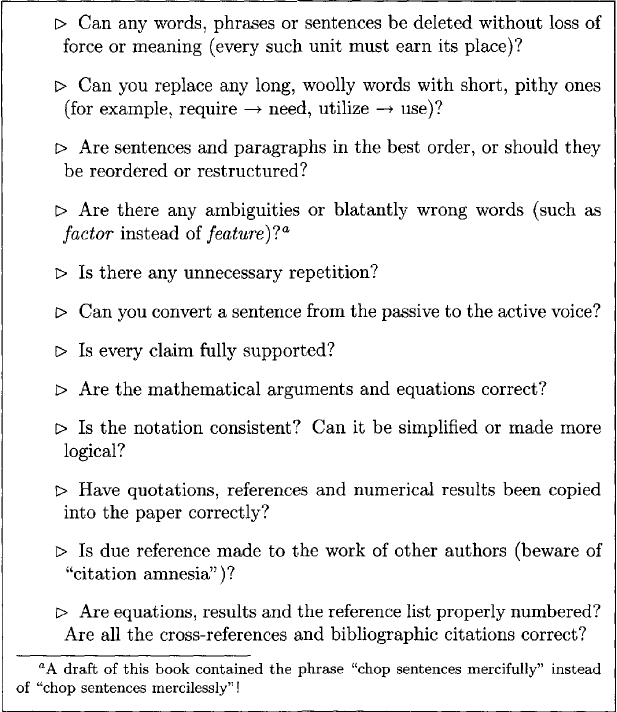
\includegraphics{figure/Figure 7.1.png}
    \caption{Checklist 1}
    \label{fig:my_label}
\end{figure}
\begin{figure}[htb]
    \centering
    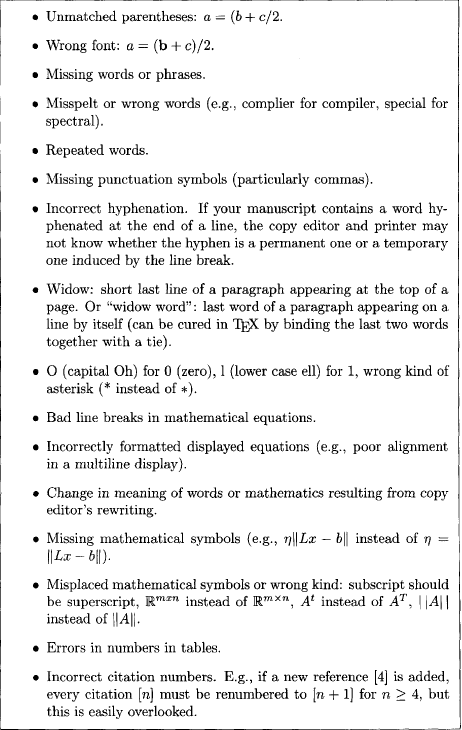
\includegraphics[width=0.9\textwidth]{figure/Figure 8.2.png}
    \caption{Checklist 2}
    \label{fig:my_label}
\end{figure}
\chapter{资料获取与写作工具}
在导师带领下开展研究时(不论是面对课程论文还是毕业设计), 我们很容易碰到以下两种情况:
\begin{enumerate}
    \item 导师给定了若干参考文献, 发来pdf论文并说``你可以先看看这些论文, 有想法可以来和我讨论";
    \item 导师提出了若干研究主题, 亲切地拍拍我们说``你可以试着了解一下这几个主题, 决定哪个比较感兴趣".
\end{enumerate}

\textbf{在本章中, 我们将}
\begin{enumerate}
    \item 首先, 介绍如何面对以上两种情况,快速了解研究主题;
    \item 其次, 介绍如何利用权威的数据库资源平台获取论文全文;
          % \item 之后, 推荐能够高效管理这些文献的开源软件 \href{https://www.zotero.org/}{Zotero};
    \item 最后, 分享能够进行在线\LaTeX 合作写作的平台 \href{https://www.overleaf.com/}{Overleaf}.
\end{enumerate}

\section{快速了解主题}
章首提到的两种情况, 对应着我们作为本科生对于目标主题不熟悉的正常现象, 是我们在研究开始时必经的锻炼与挑战. 建议大家从寻找``突破口''这一步出发, 能够帮助我们快速了解主题.

所谓``突破口'', 是指一篇\textbf{与研究主题密切相关的, 有引用其他参考文献的规范文档}. 它可以是一篇学术论文, 一本学术著作, 或是一份教师授课讲义, 只要是有\textbf{引用其他参考文献}的正式文档都可以成为我们的``突破口''. 因为他们不但将我们导向相关文章, 还会在引言等部分对相关工作进行概括性的梳理.

\begin{figure}[H]
    \centering
    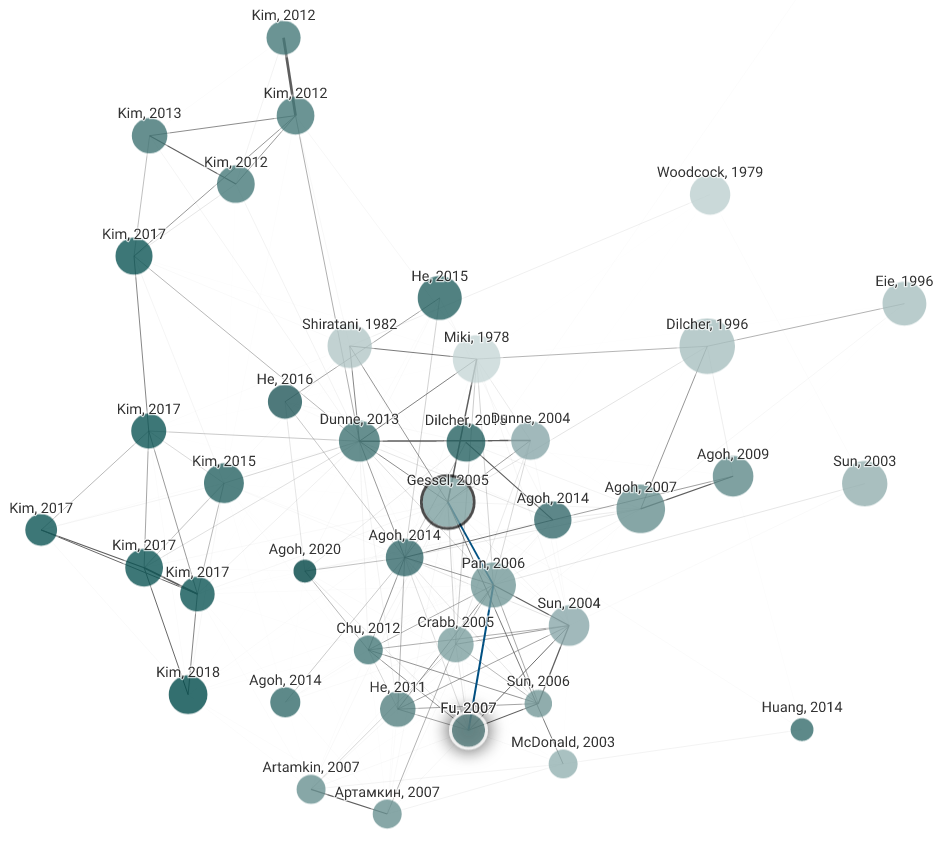
\includegraphics[width=0.8\textwidth]{figure/graph.png}
    \caption{文献~\cite{gessel_mikis_2005}与其他文献间的引用关系图}
    \label{fig:mikiGrapg}
\end{figure}

\begin{itemize}
    \item 对于第一种情况, 当导师已经提供论文时, 我们就已经有了突破口, 就能够由此进入如图~\ref{fig:mikiGrapg} 中所展示的文献引用关系图\footnote{来自: \url{https://www.connectedpapers.com/main/d08f8ead54e419058d6c88c1b2303e19e896ebaa/On-Mikis-identity-for-Bernoulli-numbers/graph}}中, 通过其参考文献追溯目标主题密切相关的高质量论文, 从而快速了解主题.
    \item 对于第二种情况, 若我们只有导师提供的关键词, 则我们需要试图寻找有引用参考文献的正式文档, 来寻找突破口. 建议采用以下步骤:
          \begin{enumerate}
              \item \textbf{借助搜索引擎(如 \href{https://www.bing.com/}{Bing} 和 \href{https://www.google.com/}{Google}, 不建议使用Baidu)直接搜索关键词}, 如果不能够直接搜到相关论文(大多数情况), 可以 寻找格式正规的学术类博客, 试着从博客中提到的参考文献找到论文或专著作为突破口. 当一篇论文在博客中被提到, 一定程度上预示着它会是一篇有影响力的好文章 (好的文章才更有可能被博客作者选出并解读).
              \item \textbf{当关键词过于笼统时, 直接搜索关键词可能得不到理想的结果, 可以尝试使用``关键词+ filetype:pdf''来限定搜索pdf文件}(如图~\ref{fig:bing} 所示). 还可以关注搜索结果中含有``.edu''的网址, 它们通常是教师上传到个人主页的讲义材料.  对我们快速了解主题具有很大帮助, 且会列出详细的参考文献.
              \item \textbf{若以上两步后仍然无法获得合适的突破口, 说明关键词依旧过于细致或笼统, 建议与老师或者其他同学沟通}, 获得更合适的关键词重新进行搜索, 或直接寻求推荐的论文.
          \end{enumerate}
\end{itemize}

\begin{figure}[H]
    \centering
    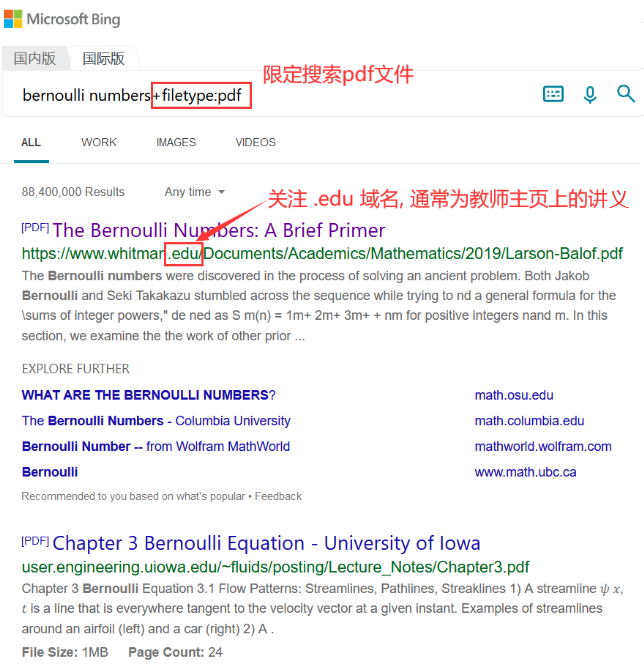
\includegraphics[width=0.75\textwidth]{figure/bingSearch.png}
    \caption{使用``关键词 + filetype:pdf''技巧在 Bing 中搜索pdf文件}
    \label{fig:bing}
\end{figure}

至此, 假设我们已经完成上述步骤, 获得了具有参考文献引用的突破口, 我们可以阅读其对于领域进展的概述, 去寻找被引用的前人文章, 并进一步关注前人文章中的引用. 由于越是相关性强的优秀的前人成果, 越有可能被其他文章所引用, 所以当我们发现一篇文章被多次引用时, 可以重点关注仔细阅读, 更加高效地了解研究主题和进展.

\section{数据库与全文获取}
在上一节中, 我们建议从``突破口''出发, 寻找其引用的参考文献. 在本节中我们将重点介绍如何获取参考文献的全文pdf, 首先将整体简述中英文数据库平台, 然后将给出一种建议的搜寻全文pdf的流程供参考.

\subsection{文献数据库平台简介}
数据库平台主要可以分为两类, 一类是全文数据库, 另一类是题录文摘数据库. 全文数据库, 顾名思义是包含文献全文的数据库, \textbf{常用的全文数据库有}:
\begin{itemize}
    \item 中文: 中国学术期刊网络出版总库(是世界上最大的连续动态更新的中国学术期刊全文数据库), 中国博士学位论文全文数据库等. 这些数据库资源都可以直接从\textbf{\href{https://www.cnki.net/}{中国知网}}\footnote{由清华大学和清华同方建于1999年, 网址为: \url{https://www.cnki.net}}获取. 而维普和万方也是两个较全面的中文全文数据库平台, 收录了大量中文文献全文, 在医学等学科领域有者各自独有的数据库. 一般直接从知网搜索即可获得大部分所需信息;
    \item 英文: 英文全文数据库可以分为两类, \textbf{一类是已发表文献数据库, 一类是预印本收录网站}:
          \begin{enumerate}
              \item \textbf{已发表英文文献数据库通常由图书馆购买}, 常用的有: ScienceDirect (涵盖了Elsevier公司出版的1800多种期刊), SpringerLink (涵盖了Springer出版的2900多种期刊), EBSCO (综合性平台, 代购买了许多子数据库), PQDT
                    (ProQuest 下的博硕学位论文库) 等;
              \item \textbf{预印本收录网站通常免费开放}, 预印本指尚未投稿或已投稿但尚未正式发表的文章, 作者可能会将未正式发表的论文全文上传至预印本网站, 表明成果的优先权并方便与同行间的及时交流. \textbf{\href{http://arxiv.org/}{arXiv}}\footnote{由物理学家 Ginsparg 建立于1991年, Cornell 大学负责运营维护, 网址为: \url{http://arxiv.org/}}是数学、物理学和计算机学科常用的预印本网站, 其他学科也有各自的预印本网站如bioRxiv(生物学), medRxiv(医学)等.
          \end{enumerate}
\end{itemize}

而题录文摘数据库通常包含文章除正文以外的所有信息(如标题, 摘要, 参考文献等), 目的是起到类似搜索引擎的\textbf{全面搜索与导航功能}, 因此通常能够包含大部分全文数据库的文章,  只需要在题录文摘数据库搜索到相应条目即可进一步导向全文数据库. 可以方便我们快速全面地搜索文章标题, 查看摘要及文献引用信息. 由于中文文献通常从知网就能完成较为完整的搜索与获取全文, \textbf{以下将主要介绍英文的题录文摘数据库}:
\begin{itemize}
    \item \textbf{综合类数据库}: 大型综合性引文索引数据库如 \textbf{\href{http://apps.webofknowledge.com/}{Web of Science}}\footnote{包含了SCI和SSCI等子库, 地址为: \url{http://apps.webofknowledge.com/}}, Scopus 等;
    \item \textbf{领域特有数据库}: 许多学科有各自特有的集成检索系统如 \textbf{\href{https://mathscinet.ams.org/mathscinet}{MathSciNet}(数学)}\footnote{由 American Mathematical Society 维护, 地址为: \url{https://mathscinet.ams.org/mathscinet}, 其使用指南可以从此处获取: \url{http://did.red/RIjz09}}, DBLP(计算机)等;
    \item \textbf{新兴的免费数据库}: 为了提供更广泛的便利, 许多科技公司建立了免费的综合类题录文摘数据库如 \textbf{\href{https://scholar.google.com/}{Google Scholar}}\footnote{由Google公司维护, 地址为: \url{https://scholar.google.com/}}, \textbf{\href{https://www.semanticscholar.org/}{Semantic Scholar}}\footnote{由 Allen Institute for Artificial Intelligence 维护, 地址为: \url{https://www.semanticscholar.org/}} 等.
\end{itemize}

故整体而言, 题录文摘数据库可以为我们提供完整的搜索功能, 当我们从中确定需要的文献后, 可以直接从文摘数据库提供的链接导向全文数据库, 从而下载全文.

\subsection{使用体验与建议}
虽然我们已经介绍了许多著名的全文数据库和题录文摘数据库, 但在日常获取文献全文的过程中, 大家可能会面临一定的选择困难. 因此, 我们将在本节中给出对于\textbf{搜索数学论文}具体而可行的搜寻流程建议.

对于中文文献, 一般从学校已购买的知网即可获取, 其他选择也只有万方和维普两家, 远比英文文献获取要方便直接, 故在此不再赘述, \textbf{以下将着重分析英文文献的获取体验与建议}:
\begin{enumerate}
    \item 首先是选择题录文摘数据库进行搜索, 根据搜索时的具体目的, 建议从以下三个数据库中进行选择:
          \begin{itemize}
              \item \textbf{\href{https://mathscinet.ams.org/mathscinet}{MathSciNet}: 追求权威性和准确性时的首选}, 如图~\ref{fig:mathscinet}, 作为数学领域特有的集成检索系统, 经测试其数学文献更新速度要比综合性数据库如 Web of Science 更加及时, 缺点是在分析引文时不够方便.
                    \begin{figure}[H]
                        \centering
                        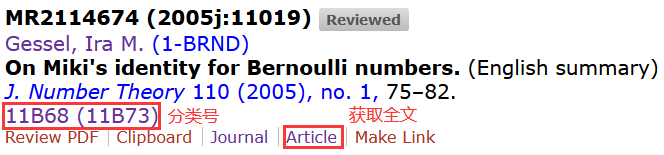
\includegraphics[width=0.8\textwidth]{figure/mathscinet.png}
                        \caption{MathSciNet 具有权威而准确的搜索结果}
                        \label{fig:mathscinet}
                    \end{figure}
              \item \textbf{\href{https://scholar.google.com/}{Google Scholar}: 需要关注全文pdf的版本时首选}, 如图~\ref{fig:googlesch}, 作为由搜索引擎提供的检索系统, 它的优势是能够汇集同一篇文章尽可能多的版本(如不同预印本和正式发表版本), 而MathSciNet等数据库一般只保留最终的发表版本(当然, 在没有特殊需求时建议阅读正式发表的版本), 但缺点也是分析引文时不够方便和众所周知的网络限制.
                    \begin{figure}[H]
                        \centering
                        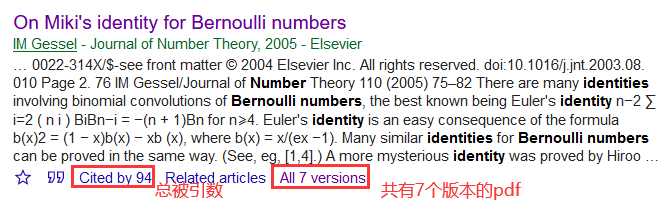
\includegraphics[width=0.8\textwidth]{figure/googlescholar.png}
                        \caption{Google Scholar 提供多个版本的全文pdf结果}
                        \label{fig:googlesch}
                    \end{figure}
              \item \textbf{\href{https://www.semanticscholar.org/}{Semantic Scholar}: 分析文章引用时首选}, 如图~\ref{fig:semantic}, 作为新兴的集成检索系统, 它能够很方便地分析文献的引用和被引, 甚至能够直接展示引用时是引用背景还是引用方法. 而且它不需要图书馆购买即可免费使用(意味着无需校园网), 但缺点是信息不如前两个数据库准确, 不建议从此处搜寻全文的pdf.
                    \begin{figure}[H]
                        \centering
                        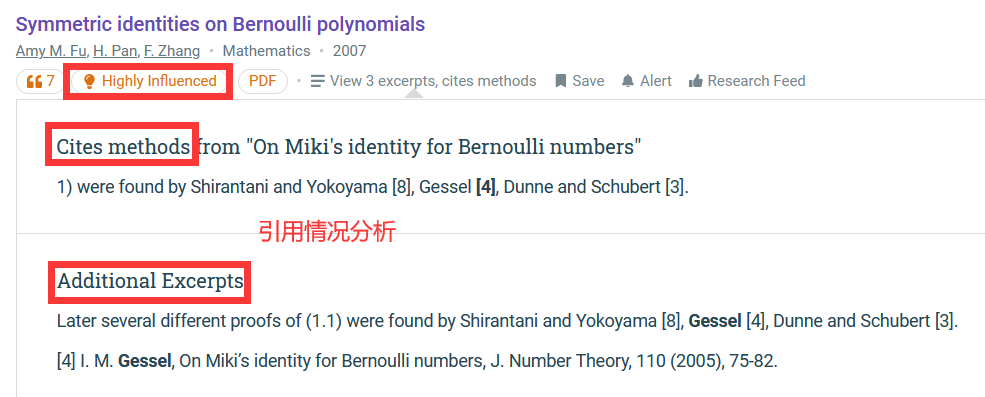
\includegraphics[width=0.8\textwidth]{figure/semantic.png}
                        \caption{Semantic Scholar 具有强大的引文分析功能}
                        \label{fig:semantic}
                    \end{figure}
          \end{itemize}
    \item 在通过题录文摘数据库进行检索并点击获取全文后, 通常我们会被导向全文数据库, \textbf{在学校图书馆已经购买该数据库时我们可以直接下载pdf, 但如果对应的数据库未被学校购买, 我们可以依次尝试以下三步获取全文:}
          \begin{itemize}
              \item \textbf{使用 \href{https://scihubtw.tw/}{Sci-Hub}\footnote{地址之一为: \url{https://scihubtw.tw/}, 可能经常变动} 解锁版权限制}, Sci-Hub 是一个能够免费获取期刊论文的平台, 也因此收到出版商的长期打压. 使用时只需要将数据库中该文章网址(上一步已经得到)粘贴进 Sci-Hub 即可自动下载全文, 当然也可以粘贴 DOI 或文章标题进行搜索.
              \item \textbf{使用 \href{https://scholar.google.com/}{Google Scholar} 搜索不同来源的全文}, 我们之前已经提到 Google Scholar 可以提供多个来源的全文pdf, 当其中的已尝试过的数据库未被学校购买时, 不妨试试其他来源.
              \item \textbf{使用 \href{https://www.bing.com/}{Bing} 等搜索引擎进行搜索}, 目前的搜索引擎已经十分发达, 在上述方法都失效时从搜索引擎搜索往往能发现在其他平台(如学院官网, 中小型数据库, 教师主页等)发布的全文pdf (不要忘记``+filetype:pdf''的技巧), 但应注意这种方法可能损失一定的权威性(可能不是最终发表版本).
          \end{itemize}
          经过笔者长期以来的测试, \textbf{$95\%$以上的文献从学校购买的全文数据库或Sci-Hub都能获取}, 且尚未出现经过以上三步后仍无法获取的情况,  欢迎读者\href{mailto:shiyuling@163.sufe.edu.cn}{交流联系}.
\end{enumerate}
此外, 下载英文电子书时也有相应的平台 \textbf{\href{https://libgen.is/}{Library Genesis}}\footnote{地址为: \url{https://libgen.is/}, 访问较为稳定} 如图~\ref{fig:libgen} 所示, 电子书版本齐全且使用方便, 大部分英文教材和出版书籍都能稳定下载, 感兴趣的读者也可以自由尝试.
\begin{figure}[H]
    \centering
    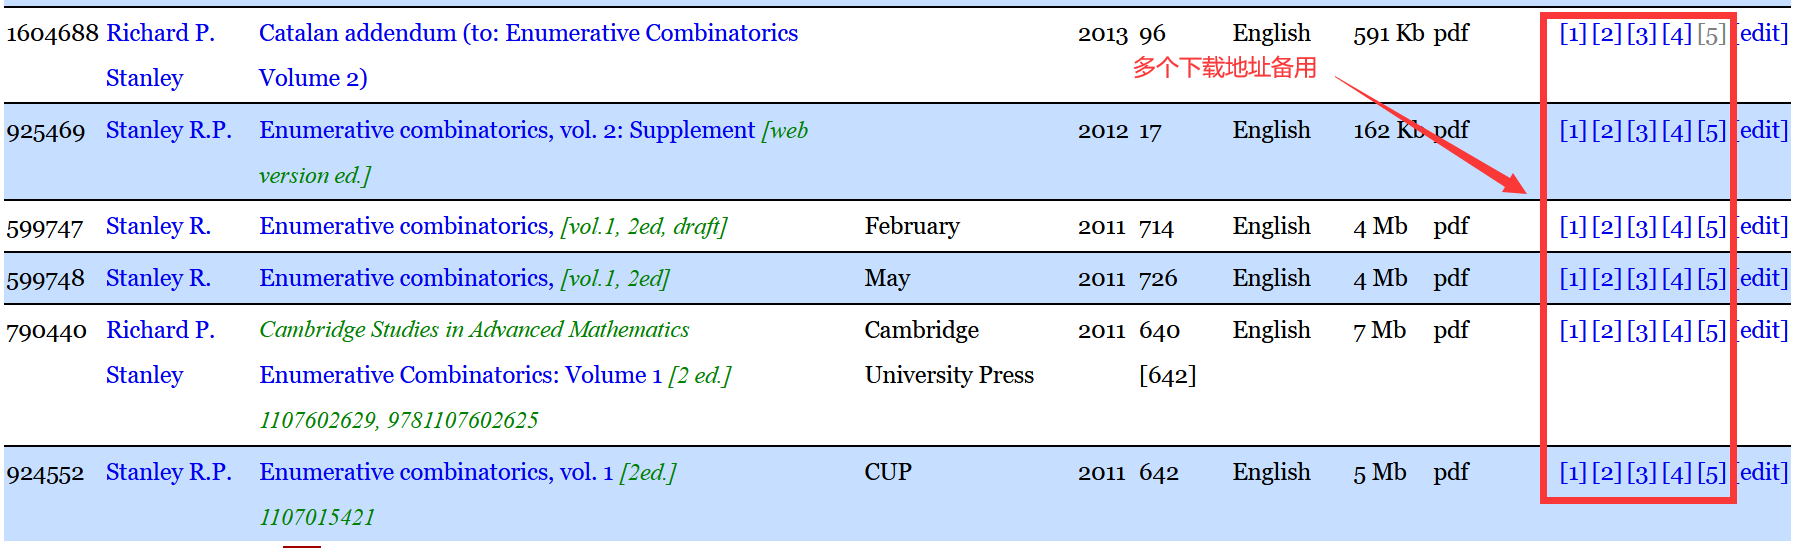
\includegraphics[width=\textwidth]{figure/ec.png}
    \caption{\textbf{\href{https://libgen.is/}{Library Genesis}} 中 \href{https://libgen.is/search.php?&req=Enumerative+Combinatorics&phrase=1&view=simple&column=def&sort=year&sortmode=DESC}{Enumerative Combinatorics} 一书的部分搜索结果}
    \label{fig:libgen}
\end{figure}
% \section{参考文献管理}

\section{在线\LaTeX 合作写作}
团队合作写作是课程论文和科研项目论文常见的写作场景, 而毕业论文而言也有与导师交流修改的合作需求, 因此利用好合作写作平台对我们的团队合作具有重要的意义. 此外, 即使是纯粹的个人项目, 我们推荐的平台也能够提供优秀的版本管理功能(例如找回之前删除的文段), 方便写作者在不同设备间迁移和备份, 防止硬盘故障和误删等意外事件造成不可挽回的损失.

在本节中, 我们要推荐的是 \href{https://www.overleaf.com/}{Overleaf}\footnote{地址为: \url{https://www.overleaf.com/}}平台. 我们将首先介绍平台的特色功能, 然后将梳理该平台的注册和使用技巧.

\subsection{主要特色功能}
\begin{figure}[H]
    \centering
    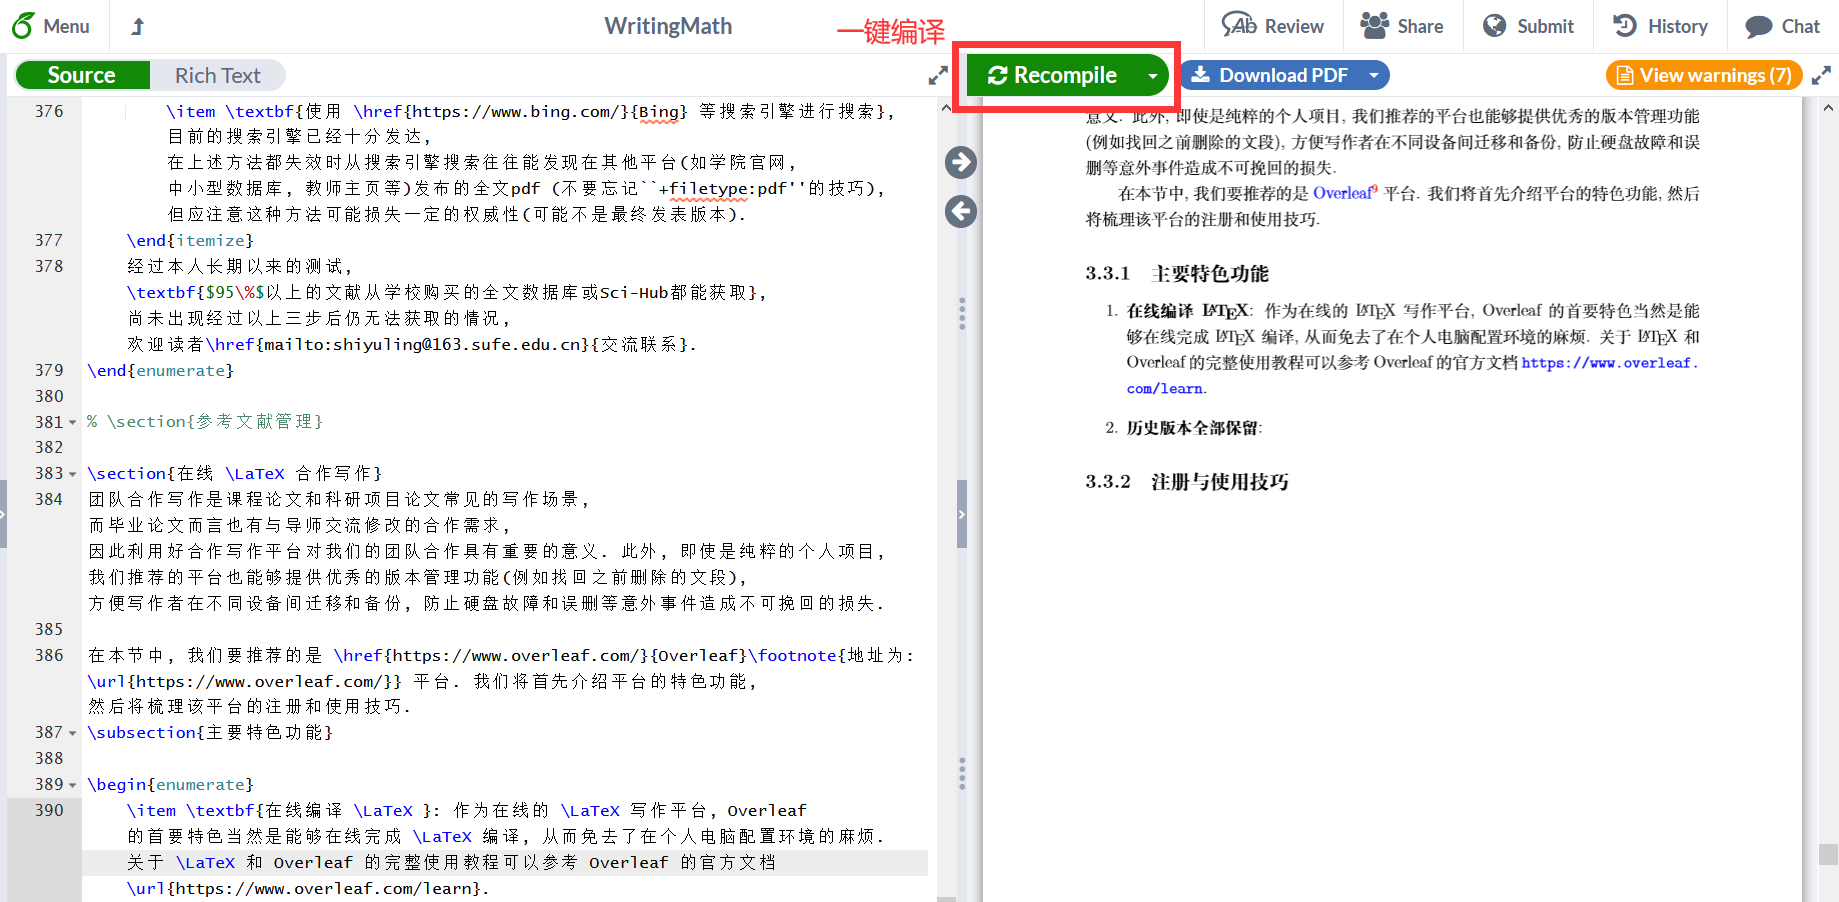
\includegraphics[width=\textwidth]{figure/overleafMain.png}
    \caption{Overleaf 主界面}
    \label{fig:overleafMain}
\end{figure}

\begin{enumerate}
    \item \textbf{在线编译\LaTeX }: Overleaf 的主界面如图~\ref{fig:overleafMain} 所示, 作为在线的\LaTeX 写作平台, 其首要特色当然是能够在线完成\LaTeX 编译, 从而免去了在个人电脑配置环境的麻烦. 关于\LaTeX 和 Overleaf 的完整使用教程可以参考 Overleaf 的官方文档 \url{https://www.overleaf.com/learn}.
    \item \textbf{编译步骤简化}: 在本地编译\LaTeX 时我们通常需要经历 pdf\LaTeX $\rightarrow$ bibtex $\rightarrow$ pdf\LaTeX $\rightarrow$ pdf\LaTeX 的编译顺序, 而在 Overleaf 上只需要在设置中选定编译器, 之后点击一次编译即可完成整个步骤. 此外, 在 Overleaf 的服务器上编译的速度也比常用的 Windows 系统上也有很大提升(但代价是需要等待 pdf 加载).
    \item \textbf{历史版本保留}: Overleaf 提供了保留文件历史版本的功能, 每一次编译时的所有文件都会被保存在历史记录中, 可以如图~\ref{fig:history} 所示方便地对比版本, 不必担心无法找回之前删除的文段.
          \begin{figure}[H]
              \centering
              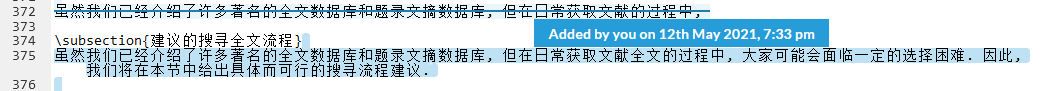
\includegraphics[width=\textwidth]{figure/history.png}
              \caption{Overleaf 中的历史版本对比}
              \label{fig:history}
          \end{figure}
    \item \textbf{与合作者交流}: Overleaf 提供了嵌入的 Chat 聊天框, 可以给合作者发送文字信息进行简单的交流, 也可以通过 Comment 功能对文件进行批注.
    \item \textbf{丰富的模板}: 除了在线编译外, Overleaf 还提供了丰富的\LaTeX 模板包括: 期刊, 报告, 简历, 书籍, 海报模板等, 如图~\ref{fig:template} 所示, 且可以直接在 Overleaf 上复制编辑, 地址为 \url{https://www.overleaf.com/gallery}.
          \begin{figure}[htbp]
              \centering
              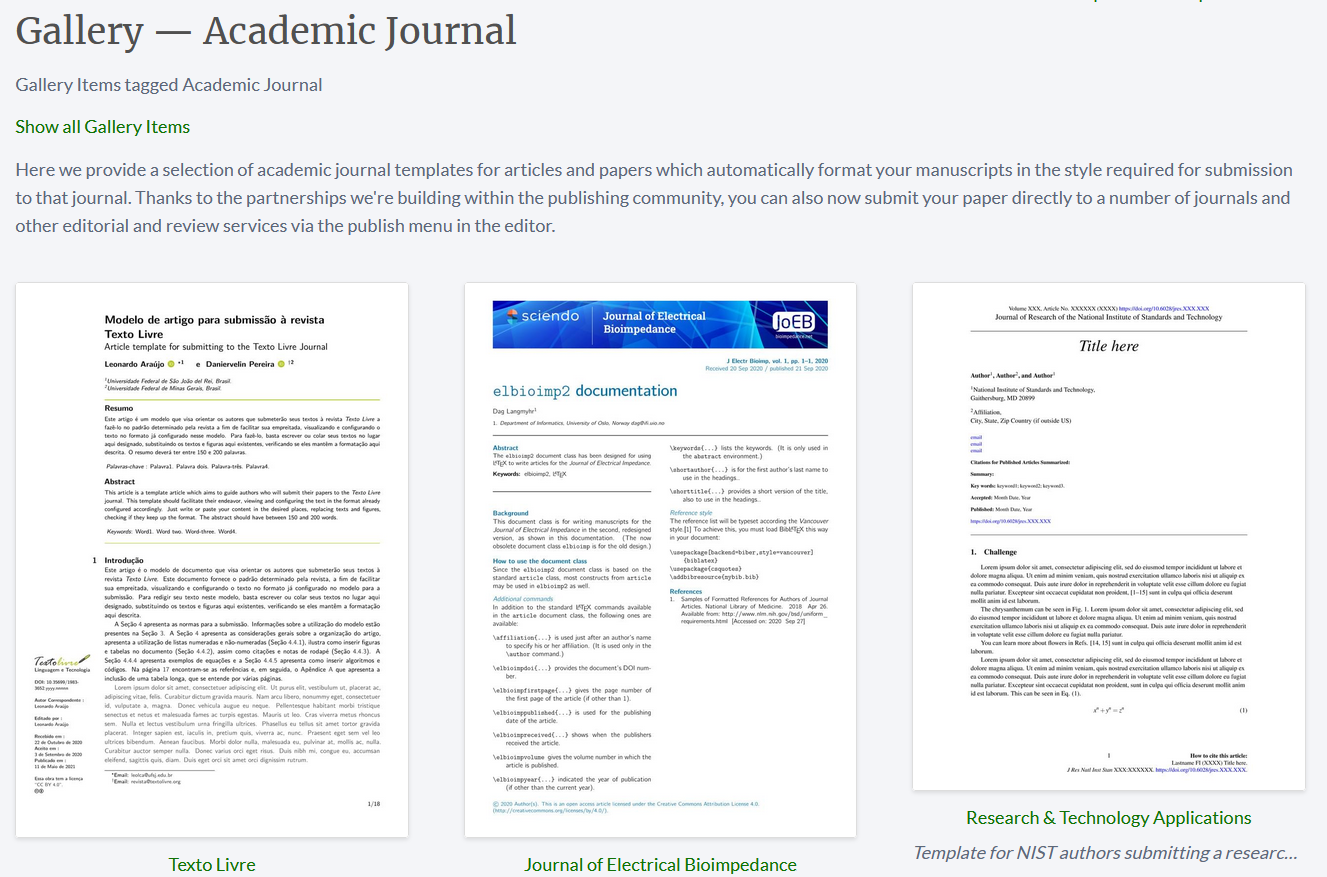
\includegraphics[width=\textwidth]{figure/template.png}
              \caption{Overleaf 还提供丰富的\LaTeX 模板}
              \label{fig:template}
          \end{figure}
\end{enumerate}

\subsection{注册与使用技巧}
我们将一份 Overleaf 注册指南放在附录~\ref{overleafGuide}, 供大家参考. 此外, 国外众多高校都有购买 Overleaf Pro, 提供更加丰富的合作与同步功能, 不知何时我财图书馆也能迈出这一步 :).

当然, 作为国外网站 Overleaf 有不可避免的缺点: 可能偶尔出现断连的情况, 但自2021年以来笔者使用时连接都很稳定, 可能是服务器情况有所改善. 读者也可以使用国内的类似平台 \textbf{\href{http://raisepub.com/}{RaisePub}}\footnote{是一个基于 Overleaf 源码开发的国内平台, 地址为: \url{http://raisepub.com/}}, 有十分稳定的连接速度和 Overleaf 的主要功能, 且目前完全免费.

\chapter{后记}\mnote{感谢老师, 可以加一些关于修改的体会(多修改 多交流)}
撰写和发表学术论文不是一件容易的事,如果你的论文被拒绝了,也许只是你这匹千里马没有遇到属于自己的伯乐,毕竟千里马常有,而伯乐不常有。在学术研究中形成自己的想法并与他人分享,是学术生活中最有意义的事之一。论文的发表、讨论往往会带来新的见解和新的合作,充分抓住这个机会。

\addcontentsline{toc}{chapter}{参考文献}
\printbibliography
\appendix
\chapter{Overleaf 注册与使用指南}\label{overleafGuide}
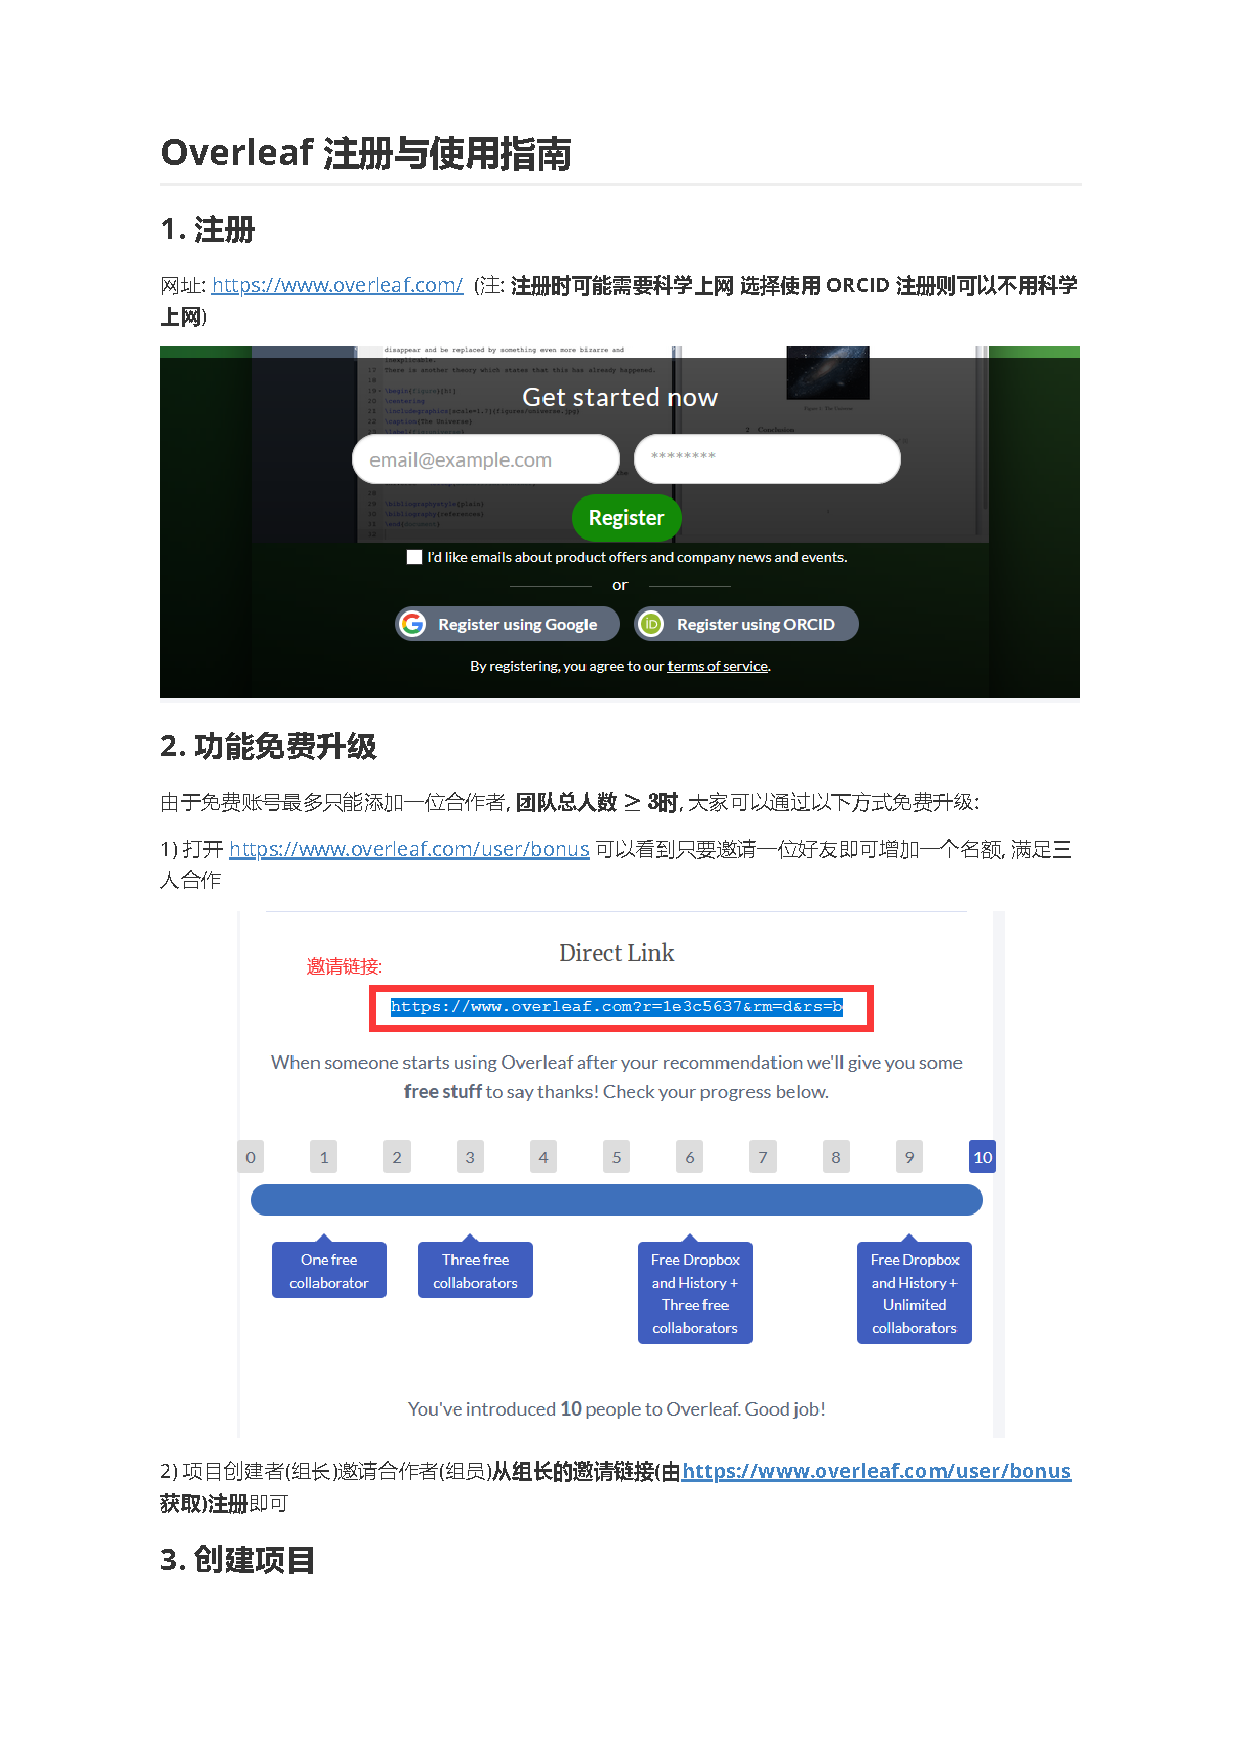
\includepdf[pages=-]{figure/OverleafGuide.pdf}
\end{document}
